\section{Ejercicio 7}
En el presente ejercicio se analiza la ejecución del siguiente código.

\lstinputlisting[language={[Motorola68k]Assembler}]{code/ej7.asm}

Del código se destaca que se inicializa al \textit{status register} con el valor \$0800. Del manual del DSP 56000 de Motorola se extrae que se activa el bit S1, lo que configura el \textit{scaling mode} en \textit{Scale Up}, lo cual produce un corrimiento del punto fraccionario hacia la derecha, aumentando la parte entera en 1 bit. 

\begin{table}[H]
\centering
\begin{tabular}{|c|c|c|}
\hline
\textbf{Dirección} & \textbf{Mapa X (origen)} & \textbf{Mapa Y (destino)} \\ \hline
\$0000             & \$10fedc                 & \$21fdb8                  \\ \hline
\$0001             & \$210fed                 & \$421fda                  \\ \hline
\$0002             & \$4210fe                 & \$7fffff                  \\ \hline
\$0003             & \$84210f                 & \$800000                  \\ \hline
\$0004             & \$d84210                 & \$b08420                  \\ \hline
\$0005             & \$fb8421                 & \$f70842                  \\ \hline
\end{tabular}
\caption{Estado de la memoria luego de correr el programa.}
\label{tab:ej7_mem}
\end{table}

En la tabla~\ref{tab:ej7_mem} se muestra el resultado de la ejecución del programa, donde se puede observar el efecto del \textit{Scale Up} ya que las posiciones de memoria en Y surgen de realizar un shift aritmético a izquierda sobre las posiciones de memoria en X, exceptuando las posiciones \$0002 y \$0003 ya que en las mismas al cargarse sobre el acumulador A e interpretarse como numero de punto fijo corresponden a números, en modulo, mayor a 1, por lo cual al intentar realizar el movimiento del acumulador al espacio de memoria actuará el limitador.

\begin{figure}[H]
    \centering
    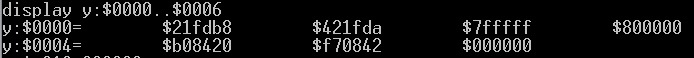
\includegraphics[width=\textwidth]{figs/ej7/1.jpeg}
    \caption{Estado final de la memoria (simulación).}
    \label{fig:ej7_mem}
\end{figure}

\begin{figure}[H]
    \centering
    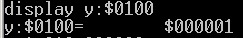
\includegraphics[width=0.5\textwidth]{figs/ej7/2.jpeg}
    \caption{Estado final de la memoria Y:\$0100 (simulación).}
    \label{fig:ej7_y100}
\end{figure}

En la figura~\ref{fig:ej7_y100} se aprecia que el valor final de la posición de memoria Y:\$0100 es 1. Observando el programa, se concluye que esta posición de memoria puede estar siendo empleada como flag para indicar si en algún momento de la ejecución existió un redondeo. 